\documentclass[a4paper,12pt]{article}

%\setlength{\parskip}{\baselineskip} % Spacing between paragraphs%
%\setlength{\parindent}{0pt} % Don't indent new paragraphs
%\everypar{\noindent\hangafter=1\hangindent=2em\relax% this to be debugged

\usepackage{multirow}
\usepackage[T1]{fontenc}
\usepackage{tikz}
% \usepackage{amssymb}  %$\because$ $\therefore$
\tikzset{
	treenode/.style = {align=center, inner sep=0pt, text centered,  font=\small},
	explored/.style = {treenode, circle, black, draw=black,  text width=1.2em},
	hid/.style = {treenode, circle, lightgray, dashed},
	pruned/.style = {treenode, circle, lightgray, dashed, draw=black, font=\sffamily\bfseries, text width=1.2em},
	expr/.style = {treenode, draw=black},
	dead/.style = {treenode, draw=black}
}


% Floating picture next to each other
\usepackage{listings}
\usepackage{floatrow}
\usepackage{subfig}
\floatsetup[figure]{style=plain,subcapbesideposition=center}

\usepackage{standalone}
\usepackage{indentfirst}
\setlength{\parindent}{2em}

% package for pseudocode format and algorithm
%\usepackage[english]{babel}
%\usepackage[utf8]{inputenc}
\usepackage{amsmath}
\usepackage{amsfonts}
\usepackage{graphicx}
\usepackage[colorinlistoftodos]{todonotes}
\usepackage{algorithm}

\usepackage[noend]{algpseudocode}
\makeatletter
\def\BState{\State\hskip-\ALG@thistlm}
\makeatother

\usepackage{graphicx}

% the overall setting of pages
\usepackage{geometry}
 \geometry{
 a4paper,
 total={210mm,297mm},
 left=20mm,
 right=20mm,
 top=25mm,
 bottom=20mm,
 }


% Title etc...
\title{COMP9101: Assignment 2}
\author{Changfeng Li (z5137858)\\
\date{12/04/2018}\\
\ UNSW\\
\ School of Computer Science and Engineering\\[-0.3ex]
\ Sydney, Australia\\
}



\begin{document}
\maketitle


%------------------------------------------------------------%
\newpage

% ---- Q1(Q)
\section*{Question 1}
% set 
\setlength{\parindent}{0pt} % Don't indent new paragraphs
\everypar{\noindent\hangafter=1\setlength{\hangindent}{1.38em}} %

(a)\textbf{[5 marks]} Revision: Describe how to multiply two $n-$degree polynomials together in $O(nlogn)$ time, using the Fast Fourier Transform (FFT). You do not need to explain how FFT works $–$ you may treat it as a black box. \\
\textit{Hint:  Remember that FFT does not multiply polynomials, what does it do? Refer to the lecture slides.}

(b)In this part we will extend the Fast Fourier Transform (FFT)algorithm described in class to multiply multiple polynomials together (not just two).\\
Suppose you have $K$ polynomials $P_1, . . . , P_K$ so that \\
\begin{center} $degree(P_1) + \cdots + degree(P_K) = S$ \end{center}

\everypar{\noindent\hangafter=1\setlength{\hangindent}{3.38em}}
\setlength{\parindent}{2em}
(i)\textbf{[5 marks]} Show that you can find the product of these $K$ polynomials in
$O(KSlogS)$ time.\\
\textit{Hint:   How  many  points  do  you  need  to  uniquely  determine  an
$S-degree$ polynomial?}

(ii)\textbf{[10 marks]} Show that you can find the product of these
$K$ polynomials in $O(SlogSlogK)$ time. Explain why your algorithm has the required time complexity.\\
\textit{Hint: consider using divide-and-conquer!}




% ---- Q1(sol)
\subsection*{Solution}
\setlength{\parindent}{0pt} % Don't indent new paragraphs


(a)

The sequence of values $\langle P_A(1), P_A(\omega_n), P_A(\omega_n ^2), . . . , P_A({\omega_n} ^ {n - 1})\rangle$, is called the \textbf{Discrete Fourier Transform (DFT)} of the sequence $A = \langle A_0,A_1,...,A_{n-1}\rangle$ which can be described in convolution form.\\
Thus, It needs several steps to complete it.

\everypar{\noindent\hangafter=1\setlength{\hangindent}{0.88em}} %

1.To multiply two polynomials $P_A(x)$ and $P_B(x)$ of degree (at most) $n$ we will evaluate them at the roots of unity of $2n+1$ orders.

2.Because \textit{FFT} is an efficient way to compute \textit{DFT} and \textit{IFFT}. This produces the \textit{DFT} of the (0 padded) sequence of their coefficients $(A_0,A_1,...,A_n,\underbrace{0,...,0}_{\text{$n$}})$. 

3.We will then multiply the corresponding values $P_A(\omega_{2n+1}^{k})$ and $P_B(\omega_{2n+1}^{k})$ . 

4.We then use the inverse transformation for \textit{DFT}, called \textit{IDFT}, to recover the coefficients of the product polynomial from its values at these roots of unity. \\


(b) (i) 
\everypar{\noindent\hangafter=1\setlength{\hangindent}{0em}} %

Suppose we have k polynomials. In average case every polynomial is of length $S/k$. But we should care about the worst case when $S \rightarrow $ "a very large number" and there exists a long polynomial whose length is near S. So under this worst case, every polynomial should add terms which are of coefficent 0, and expand to $k$ sequences of length $S$.\\
So, The detailed steps can be list below:

\begin{center} $P_A(x) = A_0 +...+{A_S}{x^S} +0\cdot x^{S+1} +...+0\cdot x^{2S};P_B(x) = B_0 +...+{B_S}{x^S} +0\cdot x^{S+1} +...+0\cdot x^{2S}$ \end{center}
\hspace{15em} $\Downarrow FFT = O(SlogS)$
\begin{center} ${P_{1}(1),P_{1}(\omega_{2S+1}),P_{1}(\omega_{2S+1}^{2}),...,P_{1}(\omega_{2S+1}^{2S})}; {P_{2}(1),P_{2}(\omega_{2S+1}),P_{2}(\omega_{2S+1}^{2}),...,P_{2}(\omega_{2S+1}^{2S})};$ \end{center}
\begin{center} $k\ numbers\ of \cdot\cdot\cdot$ \end{center}
\begin{center} ${P_{k-1}(1),P_{k-1}(\omega_{2S+1}),P_{k-1}(\omega_{2S+1}^{2}),...,P_{k-1}(\omega_{2S+1}^{2S})}; {P_{k}(1),P_{k}(\omega_{2S+1}),P_{k}(\omega_{2S+1}^{2}),...,P_{k}(\omega_{2S+1}^{2S})}.$ \end{center}
\hspace{15em} $\Downarrow Multiplication = O(KS)$
\begin{center} $\{P_{1}(1)P_{2}(1)...P_{k}(1), P_{1}(\omega_{2S+1})P_{2}(\omega_{2S+1})...P_{k}(\omega_{2S+1}), ... , P_{1}(\omega_{2S+1}^{2S})P_{2}(\omega_{2S+1}^{2S})...P_{k}(\omega_{2S+1}^{2S}) \}$ \end{center}
\hspace{15em} $\Downarrow IFFT = O(KSlogKS)$
\begin{center} $P_{final}(x) = P_{1}(x)P_{2}(x)...P_{k}(x)$ \end{center}

Thus, it can be discovered that $S \geq K$ always make sense, So convolution can be computed in time $O(KSlogKS) = O(KSlogS) + O(KSlogK) = O(KSlogS)$.\\

(b) (ii) 

If we compute these polynomials in pair everytime, For each layer, Still the time complexity of $FFT$ algorithm is still $O(SlogS)$, and we always apply divide and conquer thought on the polynomial set, Then the time copmplexity is $O(logk)$.
Thus, overall complexity is $O(logk)*O(SlogS) = O(logk*SlogS)$. 

\begin{figure}[!h]
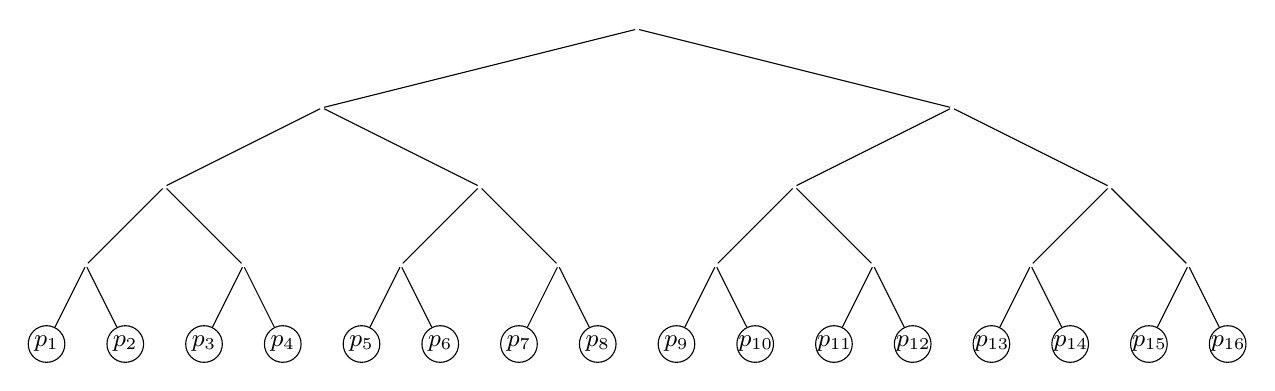
\begin{tikzpicture}[
	level/.style={level distance=1cm},
 	level 1/.style={sibling distance = 8cm},
 	level 2/.style={sibling distance = 4cm},
 	level 3/.style={sibling distance = 2cm},
 	level 4/.style={sibling distance = 1cm}
]
\node [treenode] {}
child{ node [treenode] {}
	child{ node [treenode] {}
		child{ node [treenode] {}
			child{ node [explored] {$p_1$}}
			child{ node [explored] {$p_2$}}
		}
		child{ node [treenode] {}
			child{ node [explored] {$p_3$}}
			child{ node [explored] {$p_4$}}
		}
	}
	child{ node [treenode] {}
		child{ node [treenode] {}
			child{ node [explored] {$p_5$}}
			child{ node [explored] {$p_6$}}
		}
		child{ node [treenode] {}
			child{ node [explored] {$p_7$}}
			child{ node [explored] {$p_8$}}
		}
	}
}
child{ node [treenode] {}
	child{ node [treenode] {}
		child{ node [treenode] {}
			child{ node [explored] {$p_9$}}
			child{ node [explored] {$p_{10}$}}
		}
		child{ node [treenode] {}
			child{ node [explored] {$p_{11}$}}
			child{ node [explored] {$p_{12}$}}
		}
	}
	child{ node [treenode] {}
		child{ node [treenode] {}
			child{ node [explored] {$p_{13}$}}
			child{ node [explored] {$p_{14}$}}
		}
		child{ node [treenode] {}
			child{ node [explored] {$p_{15}$}}
			child{ node [explored] {$p_{16}$}}
		}
	}
}
;
\end{tikzpicture}
\caption{}
\end{figure}












%------------------------------------------------------------%
\newpage

\section*{Question 2}

\textbf{[10 marks]} You have a set of $N$ coins in a bag, each having a value between 1 and $M$, where $M\geq N$. Some coins may have the same value. You pick two coins (without replacement) and record the sum of their values. Determine what possible sums can be achieved, in $O(MlogM)$ time.
For example, if there are $N = 3$ coins in the bag with values 1, 4 and 5 (so we could have $M = 5$), then the possible sums are 5, 6 and 9.

% ---- Q2(I)
\subsection*{Solution}
\setlength{\parindent}{0pt} % Don't indent new paragraphs
\everypar{\noindent\hangafter=1\setlength{\hangindent}{1.18em}} %



1. According to the hint, we define the value of coins as $v_1, v_2, ..., v_n$, we define the polynomial as $P(x) = x^{v_1} + ... + x^{v_n}$, with each $v_i \leq v_n$, if $v_i$

2. We multiply $P$ with itself. We can use the algorithm we have talked about in Question 1 to solve this step and get the result with $2n+1$ terms as $Q(x) = a_0 + a_1x + a_2x^2... + a_{2n}x^{2n}$, We note as a sequence $\langle a_0, a_1,...,a_{2n} \rangle$

3. We traverse the element in the sequence, if $a_i > 1(1 \leq i \leq 2n)$, then the corresponding item $a_i$ should be added to the set of possible sums.\\

\everypar{\noindent} %

For instance, if there are $N = 4$ coins in the bag with values 1, 1, 4 and 5, we can write down a polynomial $P(x) = 0 + 2x + 0\cdot x^2 + 0\cdot x^3 + x^4 + x^5$, we compute the multuplication of $P$ and itself, we get the result $Q(x) = 0 + 0\cdot x + 4\cdot x^2 + 0\cdot x^3 + 0\cdot x^4 +4\cdot x^5 + 4\cdot x^6 + 0\cdot x^7 + 1\cdot x^8 + 2\cdot x^9 + 1\cdot x^{10}$.\\
The sequence is $\langle 0, 0, 4, 0, 0, 4, 4, 0, 1, 2, 1 \rangle$
We can observe which item's coefficient $\geq$ 2 in this result polynomial, therefore, the possible sums are 2, 5, 6 and 9, that's how the algorithm works. 






%------------------------------------------------------------%
\newpage

\section*{Question 3}

Let us define the Fibonacci numbers as $F_0 = 0, F_1 = 1$ and $F_n = F_{n-1} +F_{n-2}$ for all n $\geq$ 2. Thus, the Fibonacci sequence looks as follows: 0, 1, 1, 2, 3, 5, 8, 13, 21, ...

(a)\textbf{[5 marks]} Show, by induction or otherwise, that 
\[
\begin{bmatrix}
F_{n+1} & F_{n}\\
F_{n} & F_{n-1}
\end{bmatrix}
=
\begin{bmatrix}
1 & 1\\
1 & 0
\end{bmatrix}
^n \] 
for all integer n $\geq$ 1.

(b)\textbf{[10 marks]}
Hence or otherwise, give an algorithm that finds $F_n$ in $O(logn)$ time.\\
\textit{Hint:  You may wish to refer to Example 1.5 on page 28 of the "Re-view Material" found as lecture notes for Topic 0 on the Course Resources page of the course website.}




\subsection*{Solution}
\setlength{\parindent}{0pt} % Don't indent new paragraphs

(a) Use Induction method to prove this equation is true.
We define 
\[ A(n) = 
\begin{bmatrix}
F_{n+1} & F_{n}\\
F_{n} & F_{n-1}
\end{bmatrix}
;
M = 
\begin{bmatrix}
1 & 1\\
1 & 0
\end{bmatrix}
\] 

Step1:\ 
When $n = 1$, the equation always holds obviously.

Step2:\ 
We assume that when $n = k$ always holds.\\
Now let $n = k+1$, We multiply $A(k)$ with $M$
\[
\begin{bmatrix}
F_{k+1} & F_{k}\\
F_{k} & F_{k-1}
\end{bmatrix}
\begin{bmatrix}
1 & 1\\
1 & 0
\end{bmatrix}
=
\begin{bmatrix}
F_{k+1} + F_{k} & F_{k+1}\\
F_{k} + F_{k-1} & F_{k}
\end{bmatrix}
=
\begin{bmatrix}
F_{k+2} & F_{k+1}\\
F_{k+1} & F_{k}
\end{bmatrix}
= A(k+1)
 \] 

Because based on the assumption. We can draw a conclusion that 
\[
\begin{bmatrix}
F_{n+2} & F_{n+1}\\
F_{n+1} & F_{n}
\end{bmatrix}
=
\begin{bmatrix}
1 & 1\\
1 & 0
\end{bmatrix}
^n  
\begin{bmatrix}
1 & 1\\
1 & 0
\end{bmatrix}
=
\begin{bmatrix}
1 & 1\\
1 & 0
\end{bmatrix}
^ {n+1}\]
always hold as well, which is perfectly proved.

(b) 
For the matrix equation 
\[ A(n) =
\begin{bmatrix}
F_{n+1} & F_{n}\\
F_{n} & F_{n-1}
\end{bmatrix}
=
\begin{bmatrix}
1 & 1\\
1 & 0
\end{bmatrix}
^n \] 
We consider two cases:\\
1. When $n$ is a odd number
\[ A(n) = A(\frac{n}{2}) * A(\frac{n}{2}) * A(1) =
\begin{bmatrix}
1 & 1\\
1 & 0
\end{bmatrix} ^{\frac{n}{2}} 
\begin{bmatrix}
1 & 1\\
1 & 0 
\end{bmatrix} ^{\frac{n}{2}}
\begin{bmatrix}
1 & 1\\
1 & 0
\end{bmatrix}
\]
2. When $n$ is an even number
\[ A(n) = A(\frac{n}{2}) * A(\frac{n}{2}) =
\begin{bmatrix}
1 & 1\\
1 & 0
\end{bmatrix} ^{\frac{n}{2}} 
\begin{bmatrix}
1 & 1\\
1 & 0 
\end{bmatrix} ^{\frac{n}{2}}
\]
Thus $A^n = A^{n/2}A^{n/2} = \textstyle\prod\limits_1^n A^1$ .So calculate $A^n$ matrix, we should calculate $A^{n/2}$  matrix and multiply it by itself. To calculate $A^{n/2}$ we would have to do the same with $A^{n/4}$ and recursively so on. Obviously, the tree height is $log_2(n)$.
Therefore, we can perform the multiplication of two matrices in any power $O(1)$. We should perform $log_2(n)$ of such multiplications. So complexity satisfy $O(logn)$









%------------------------------------------------------------%
\newpage

\section*{Question 4}

\textbf{[10 marks]} You have $N$ items for sale, numbered from 1 to $N$. Alice is willing to pay $a[i] > 0$ dollars for item $i$, and Bob is willing to pay $b[i] > 0$ dollars for item $i$, Alice is willing to buy no more than $A$ of your items, and Bob is willing to buy no more than B of your items. Additionally, you must sell each item to either Alice or Bob, but not both, so you may assume that $N \leq A + B$. Given $N, A, B, a[1..N]$ and $b[1..N]$, show that you can determine the maximum total amount of money you can earn in $O(NlogN)$ time.\\
\textit{Hint:  Suppose $N = A + B$ and pretend you wish to sell all items to Alice, but must choose
$B$ of  them  to  give  to  Bob  instead. Which ones do you want to give to Bob first? Then extend your approach to handle $N < A + B$ as well.}

\subsection*{Solution}

1. Build up a list $Dif[]$ which stores the abs of difference of $a[i]$ and $b[i]$,that is $Dif[i]=ABS(a[i]-b[i])$. Time complexity = $O(N)$

2. Sort $Dif$ by decending order. Record their corresponding $i$ with their difference together. Time complexity = $O(NlogN)$

3. Traversing the list $Dif$, for current difference and $i$ go back to list $A$ and $B$ and compare $a[i]$ and $b[i]$, Time complexity = $O(N)$

if $a[i] >= b[i]$: 

if $A>0$, then we sell item i to $A$, $A = A - 1$, and append $A[i]$ to my selection list $S$.

if $A=0$ and $B>0$, then we sell item i to $B$, $B = B - 1$, and append $B[i]$ to my selection list $S$.\\

if $a[i] < b[i]$:

if $B>0$, then we sell item i to $B$, $B = B - 1$, and append $B[i]$ to my selection list $S$.

if $B=0$ and $A>0$, then we sell item i to $A$, $A = A - 1$, and append $A[i]$ to my selection list $S$.\\

else:
all of the N items I owned have been sold out. Stop the algorithm.

4. Compute the maximum total number $sum(S)$, this result is a maximum money I can earned.\\

Time complexity = $O(N) + O(NlogN) + O(N) = O(NlogN)$










%------------------------------------------------------------%
\newpage

\section*{Question 5}

Your army consists of a line of $N$ giants, each with a certain height. You must designate precisely $L \leq N$ of them to be leaders. Leaders must be spaced out across the line; specifically, every pair of leaders must have at least $K \leq 0$ giants standing in between them. Given $N, L, K$ and the heights $H[1..N]$ of the giants in the order that they stand in the line as input, find the maximum height of the shortest leader among all valid choices of $L$ leaders. We call this the $optimisation$ version of the problem.\\
For instance, suppose $N = 10, L = 3, K = 2$ and $H = [1, 10, 4, 2, 3, 7, 12, 8, 7, 2]$. Then among the 10 giants, you must choose 3 leaders so that each pair of lead-ers has at least 2 giants standing in between them. The best choice of leaders has heights 10, 7 and 7, with the shortest leader having height 7. This is the best possible for this case.

(a)\textbf{[10 marks]} In the decision version of this problem, we are given an additional  integer $T$ as input. Our task is to decide if there exists some valid choice of leaders satisfying the constraints whose shortest leader has height no less than $T$. Give an algorithm that solves the decision version of this problem in $O(N)$ time.

(b)\textbf{[10 marks]} Hence, show that you can solve the optimisation version of this problem in $O(NlogN)$ time.

\subsection*{Solution}
\setlength{\parindent}{0pt} % Don't indent new paragraphs

We mark $L$ = \#Leader, $N = len(H)$, $K$ is the interval between $L$.

(a)

1. Build a new list $L_p$ to record possible leaders. 

2. Traverse the list $H$, If we find a number $H[i] >= T$, Append this number $H[i]$ to $L_p$, $L = L - 1$.

3. After procedure 2, we jump $k$ numbers in $L$, continue looping procedure a2 until $L = 0$.

Time Complexity is $O(n)$.

(b)

1. Build a new list $L_{sorted}$.

2. Apply $MergeSort$ algorithm to sort $H$ in descending order and save the result to $L_{sorted}$. Complexity is $O(nlogn)$.

3. Apply $BinarySearch$ algorithm to $L_{sorted}$ until I find the first number $L_{sorted}[j] >= T$ in $L_{sorted}$, then we define $T = H[j]$. Complexity is $O(nlogn)$.

4. apply the procedures introduced in (a), if value of $T$ make (a) successfully executed (It means $L$ successfully decrease to 0, we have found $L$ nums of leaders), then $N = \frac{N}{2}$ and repeat procedure b3. else expand $N = \frac{N}{4} + \frac{N}{2}$ and ..., until the answer was finally computed.\\

Time complexity $O(logn)*O(n) = O(nlogn)$



%------------------------------------------------------------%


\end{document}